\chapter{Experiments}
\label{chapter_experiments}

\section{Performance Analysis}

Experiments are performed on a high-end PC with Intel i7-2600 and NVIDIA GeForce GTX560Ti. The frame rate of the application varies, depending on the complexity of the apparel mesh and whether the avatar is female or male. If the apparel mesh contains a large number of vertices, the physics simulation takes more time and the frame rate drops. The accessories of the female mesh such as the hair and earrings are very highly detailed and cause a considerable drop in the frame rate. The minimum acceptable frame rate is 120 frames per second(fps), which is set as the simulation rate of the physics environment. Two sets of frame rates across the simulation can be seen in Figure~\ref{fig:fps}. Notice the common pattern in both of the simulations. The first drop corresponds to the start of the animation of the avatar with the input from depth sensor. Until that point, the avatar is static, the motion filters do not run and the simulation runs at a higher speed. Approximately 600 FPS is lost due to the motion filtering and skinning. The first cliff in the graph corresponds to the point where the physics simulation is stopped. The second cliff starts when the input from the depth sensor is stopped and the simulation is stagnant.  

\begin{figure}[htbp]
	\begin{center} 
	\fbox{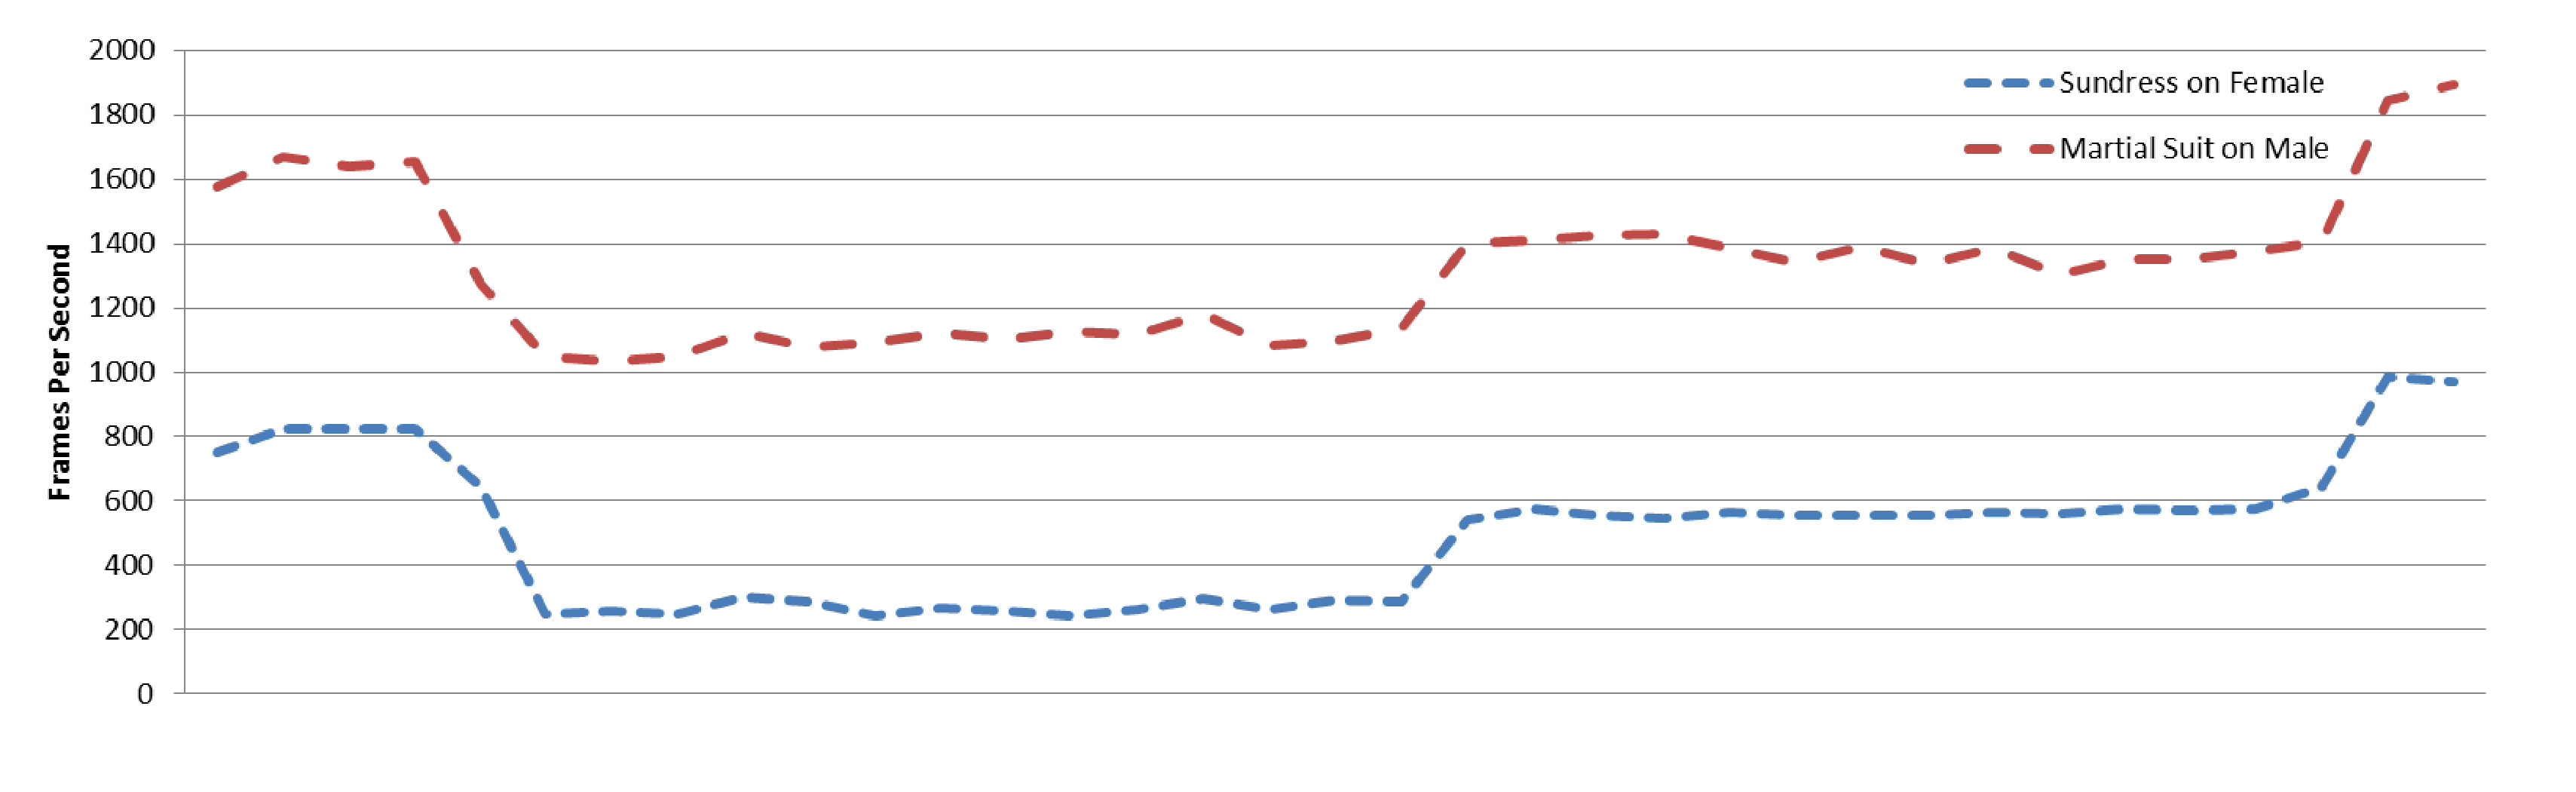
\includegraphics[width=1.00\textwidth]{./figures/fps.eps}}
	\end{center}
	\caption{The frame rate for two different apparel meshes.}
	\label{fig:fps}
\end{figure}

Aside from the overall motion smoothing, the main motion filters are dominant over the arms and the legs. The effects of motion filtering and smoothing on the arm can be seen in Figures~\ref{fig:forearm-comparison}~and~\ref{fig:rotation-filter}. The filters on the legs focus on solving the foot skating problem. The corrected displacement values can be seen in Figure \ref{fig:footskating}. The virtual unit is the unit step in the virtual world. For reference, the virtual avatars' height is 55 virtual units. Hence, a virtual unit corresponds close to 20 cm, which is a significant foot skating error.  


\begin{figure}[htbp]
	\begin{center} 
	\fbox{\includegraphics[width=1.00\textwidth]{./figures/footskate.eps}}
	\end{center}
	\caption{The corrected displacement of feet.}
	\label{fig:footskating}
\end{figure}

The measurement process to identify the body parameters starts after a subject is recognized, identified and calibrated for tracking. Following the parameter estimation, the virtual avatar and cloth are created and the simulation starts. The total time for the measurement of body parameters and resizing the cloth does not exceed 1.005 seconds. Considering the time for acquiring 30 frames of input from the depth sensor is 1.0 second, it is safe to say that the measurement algorithm does not introduce any delays for a real time application because it needs to run only once at the beginning of the simulation. The body sizes are estimated with error rates less than 4\%, which is sufficient for the realism of the simulation and determining the appropriate apparel size. Table~\ref{tbl:body_results} presents the measurements of the body dimensions, as well as the errors and standard deviations of the measurements in 30 frames for three subjects. The results are compared with the results from~\cite{Giovanni2012} and \cite{Samejima2012}, which are also real-time applications, in Table~\ref{tbl:performance_compare}.

\begin{table}
\begin{center}
\begin{tabular}{|c|c|c|c|c|c|c|c|c|}
\hline
  & \multicolumn{4}{c|}{\textbf{Shoulder Width (cm)}} & \multicolumn{4}{c|}{\textbf{Body Height (cm)}} \\ \hline
  \rotatebox{90}{Subject } & \rotatebox{90}{Real } & \rotatebox{90}{Estimated } & \rotatebox{90}{Error (\%)} & \rotatebox{90}{Deviation } & \rotatebox{90}{Real } & \rotatebox{90}{Estimated } & \rotatebox{90}{Error (\%)} & \rotatebox{90}{Deviation } \\ \hline
 1 & 43 & 43.6 & 1.0 & 7.8 & 172 & 170.8 & 0.6 & 2.5  \\ \hline
 2 & 46 & 44.3 & 3.0 & 8.5 & 176 & 172.1 & 2.0 & 1.4  \\ \hline
 3 & 51 & 48.8 & 4.0 & 12.1 & 176 & 174.0 & 1.0 & 6.6  \\ \hline
 4 & 48 & 50.0 & 4.0 & 2.5 & 188 & 191.0 & 1.5 & 7.1  \\ \hline
 5 & 44 & 42.6 & 3.0 & 4.2 & 178 & 175.8 & 1.2 & 3.1  \\ \hline
\end{tabular}
\end{center}
\caption{Performance figures for five different subjects.}
\label{tbl:body_results}
\end{table} 

\begin{table}
\begin{center}
\begin{tabular}{|l|c|c|c|c|} 
\hline 
  & \rotatebox{90}{\parbox[c]{2.95cm}{\mbox{Error Average} \mbox{\hspace{0.7cm}(\%)}}} & \rotatebox{90}{\parbox[c]{2.95cm}{\mbox{Error Deviation} \mbox{\hspace{0.7cm}(\%)}}} & \rotatebox{90}{Duration} & \rotatebox{90}{Estimation} \\ \hline
  Our Approach & 2.13  & 1.20   & 1.00 & Fixed \\ \hline 
  Giovanni et al.~\cite{Giovanni2012}  & 4.00  & 3.00  & 1.00 & None \\ \hline
  Samejima et al.~\cite{Samejima2012}  & 6.72  & 4.68  & n/a & PCA \\ \hline
\end{tabular}
\end{center}
\caption{Performance comparison with \cite{Giovanni2012} and \cite{Samejima2012} regarding height measurements.}
\label{tbl:performance_compare}
\end{table}

For the collision spheres, the quality of the results can be assessed by the smoothness of the collision simulation,  as seen in Figure \ref{fig:system}. Throughout the simulation, unnatural intersections between the cloth and the avatar never take place, while the cloth appears to rest on the skin naturally, without space between the two meshes. Figure~\ref{fig:examples} shows examples of three garments on a model with different postures generated with our implementation. The six apparel meshes, three for female avatar and three for male avatar can be seen in Figure~\ref{fig:apparels}.

\begin{figure}[htbp]
	\begin{center} 
	\includegraphics[width=1.00\textwidth]{./figures/scshot.eps}
	\end{center}
	\caption{An example depth map data and the corresponding posture of the subject with a virtual cloth on it.}
	\label{fig:system}
\end{figure}
 
 \begin{figure}[htbp] 
	\centerline{
	\includegraphics[width=0.250\textwidth]{./figures/sundress1.eps}
	\includegraphics[width=0.250\textwidth]{./figures/sundress2.eps}
	\includegraphics[width=0.250\textwidth]{./figures/sundress3.eps}
	\includegraphics[width=0.250\textwidth]{./figures/sundress4.eps}
	}
	\centerline{(a)}
	\centerline{\ }
	\centerline{
	\includegraphics[width=0.250\textwidth]{./figures/jeans-1.eps}
	\includegraphics[width=0.250\textwidth]{./figures/jeans-2.eps}
	\includegraphics[width=0.250\textwidth]{./figures/jeans-3.eps}
	\includegraphics[width=0.250\textwidth]{./figures/jeans-4.eps}
	}
	\centerline{(b)}
	\centerline{\ }
	\centerline{
	\includegraphics[width=0.250\textwidth]{./figures/flightsuit-1.eps}
	\includegraphics[width=0.250\textwidth]{./figures/flightsuit-2.eps}
	\includegraphics[width=0.250\textwidth]{./figures/flightsuit-3.eps}
	\includegraphics[width=0.250\textwidth]{./figures/flightsuit-4.eps}
	}
	\centerline{(c)}
	\caption{Examples of different garments on a model with different postures: (a) sun dress, (b) jeans and vest, and 	(c) flight suit.}
	\label{fig:examples}
\end{figure}


\begin{figure}[htbp] 
	\centerline{
	\includegraphics[width=0.333\textwidth]{./figures/sundress.eps}
	\includegraphics[width=0.333\textwidth]{./figures/jeans.eps}
	\includegraphics[width=0.333\textwidth]{./figures/flight.eps}
	}
	\centerline{(a)}
	\centerline{\ }
	\centerline{
	\includegraphics[width=0.333\textwidth]{./figures/shirt.eps}
	\includegraphics[width=0.333\textwidth]{./figures/duster.eps}
	\includegraphics[width=0.333\textwidth]{./figures/martial.eps}
	}
	\centerline{(c)}
	\caption{The designed apparel meshes for the male and female avatars.}
	\label{fig:apparels}
\end{figure}
